\documentclass{article}
% Results-focused third draft; main_v2.tex is preserved.
% Main-v3 figures and numerical provenance: Graphs/main_v3/README.md.
% Author annotations are hidden; revision text is rendered without color.
% Exact-loss tables: docs/reports/v24_optimizer_search_2026-09-10.{pdf,csv,sources.json}
% and docs/reports/v24_mamba_lr_di_10day_2026-09-14.{pdf,csv,sources.json}.
% Figure data and reproducible generator: Graphs/main_v2/README.md.

% Official ICLR 2027 submission template.
% Keep anonymous review mode. Enable only for an accepted camera-ready paper.
\usepackage{iclr2027_conference,times}
% \iclrfinalcopy

\usepackage[utf8]{inputenc} % allow utf-8 input
\usepackage[T1]{fontenc}    % use 8-bit T1 fonts
\usepackage{hyperref}       % hyperlinks
\usepackage{url}            % simple URL typesetting
\usepackage{booktabs}       % professional-quality tables
\usepackage{amsfonts}       % blackboard math symbols
\usepackage{nicefrac}       % compact symbols for 1/2, etc.
\usepackage{microtype}      % microtypography
\usepackage{xcolor} 
% colors
\usepackage{amsmath,amssymb,amsthm,mathrsfs,mathtools,bm}
\usepackage{graphicx}
\usepackage{subcaption}
\usepackage{placeins}

% User writing suggestions are annotations, not instructions to rewrite prose.
\newcommand{\suozhi}[1]{}
\newcommand{\lh}[1]{}
\newcommand{\codexedit}[1]{#1}
\newenvironment{codexrevision}{\begingroup}{\par\endgroup}
% Keep compatibility with existing clean-preview builds.
\ifdefined\hideauthorcomments
    \renewcommand{\suozhi}[1]{}
\fi

\title{GraphCast--Mamba: Learning Non-Markovian Corrections for Weather Forecasting}


% The \author macro works with any number of authors. There are two commands
% used to separate the names and addresses of multiple authors: \And and \AND.
%
% Using \And between authors leaves it to LaTeX to determine where to break the
% lines. Using \AND forces a line break at that point. So, if LaTeX puts 3 of 4
% authors names on the first line, and the last on the second line, try using
% \AND instead of \And before the third author name.


\author{
}


\begin{document}


\maketitle

% suozhi 原话：标题应该强调 mamba 能 capture 这些，现在标题太 general 了。
% \suozhi{The title is too general. Please name Mamba explicitly and emphasize its ability to capture non-Markovian effects in weather prediction.}

\begin{abstract}
{Unresolved atmospheric processes can introduce history dependence beyond the short input windows used by many weather forecasting models. We introduce GraphCast--Mamba, which augments a frozen, pretrained \(1^\circ\) GraphCast backbone with a trainable Mamba correction branch combining graph message passing and Mamba layers. The branch retains a temporal memory state across successive six-hour forecast steps, learning corrections informed by temporal context beyond GraphCast's two-frame input. Training is confined to the correction branch, using ERA5 data from 2015--2021. After only 2,500 optimizer updates, including warm-up, the selected model achieves substantial improvements relative to the uncorrected GraphCast backbone. It reduces the {GraphCast loss (normalized weighted mean-squared error; MSE)} by 16.3\% when aggregated over the full ten-day forecast and by 23.68\% at day 10 (240\,h after forecast initialization). At this final forecast lead time, root-mean-square error (RMSE) decreases by 10.2--17.1\% across all 11 evaluated variable groups, spanning temperature, wind, pressure, geopotential, specific humidity, and precipitation. Separate memory-reset controls support a contribution from persistent temporal context beyond additional trainable capacity. These results demonstrate broad improvements in ten-day weather forecasts through a short correction-training schedule while retaining the pretrained backbone.}
% suozhi 原话：我觉得 abstract 太短。
% \par\suozhi{The abstract is too short and should be expanded.}
% % suozhi 原话：很多名词比如 day ten 没有解释清楚。
% \par\suozhi{Please explain terms such as ``day ten'' at their first occurrence so readers can understand the forecast horizon.}
% \par\suozhi{Please foreground cheap and fast training, the approximately 16\% aggregate and 23\% final-lead loss reductions, and the roughly 10--15\% per-variable RMSE reductions. Emphasize the breadth of improvement across variables, define exactly what ``day ten'' means, and make the strength of the results clear.}
\end{abstract}



\section{Introduction}
% Turbulent flows are known as a notoriously difficult framework for numerical simulations. One of the common method in such simulations is the \textit{direct numerical simulations} (DNS) that discretize the Navier-Stokes equation to a space and time grid and then simulate directly. Such discretizations, however require a very fine grid resolution scaling as $N_{\textrm{grid}} \sim \left(Re\right)^{\alpha}$ with $\alpha \sim 2.05 $ \cite{yang2021grid}. Insufficient small-scale resolution may leave mean dissipation and enstrophy approximately converged while substantially underestimating high-order moments of velocity gradients, dissipation, and enstrophy, as well as the tails of velocity-gradient distributions and statistics involving second velocity derivatives \cite{DonzisResolutionEffects}.
%  While this becomes expensive, a variety of models that regularize the equations on a larger scale, introducing proper dissipative terms at the cost of short time accuracy \cite{Wilson1996Review}. Another approach consists in keeping coarse-grained scales, without non-controlled dissipative approximation, but at a cost of keeping the non-Markovian memory terms \cite{YenTingLinMZ2021,de2026data}.

% In this article, we investigate learned memory corrections for weather prediction by augmenting a frozen GraphCast model with a trainable branch that combines spatial message passing and temporal memory.


{Learned global weather models produce skillful forecasts from one or a few recent atmospheric states~\citep{bi2023pangu,lam2023graphcast,chen2023fuxi}. GraphCast, for example, uses two states six hours apart to predict the next state. These inputs provide only a partial description of the atmosphere: they contain a limited set of variables at finite spatial resolution, while unresolved processes can still influence their evolution. The history of the resolved state may carry information about these influences that a short input window does not capture.}

{This is a familiar closure problem in turbulent-flow modeling. Resolving the smallest dynamically active scales is computationally costly~\citep{yang2021grid}, so practical models must account for their effects on the resolved scales. A common approach uses approximate dissipative closures, such as eddy viscosity or hyperviscosity, to represent transfer to unresolved scales. These closures can reproduce selected aspects of the flow, but their accuracy depends on the quantity and scale of interest. For example, in forced two-dimensional turbulence, viscous, hyperviscous, and Leith closures can approximate enstrophy transfer, whereas the Smagorinsky closure dissipates enstrophy at the wrong scales~\citep{pietarila2013closures}. Resolution studies provide a related caution: mean dissipation and enstrophy can be nearly converged while higher-order moments of velocity gradients, dissipation, and enstrophy, together with distribution tails, remain substantially underestimated~\citep{DonzisResolutionEffects}. Reproducing bulk statistics therefore does not ensure accurate fluctuations or extreme events.}

{A complementary approach allows the closure to depend on the history of the resolved state. Unresolved variables have their own dynamics, so their influence need not be determined by the current resolved variables alone; past observations can contain information about those hidden degrees of freedom. The Mori--Zwanzig formalism makes this explicit: eliminating unresolved variables generally yields an instantaneous term, a history-dependent memory term, and a term associated with unresolved initial conditions, even when the full dynamics are Markovian~\citep{YenTingLinMZ2021,de2026data}. Retaining the memory contribution leads to a \emph{non-Markovian} closure, in which the resolved evolution depends on past states as well as the present one. This motivates persistent temporal memory as a mechanism for representing unresolved influences that an instantaneous dissipative approximation may miss.}

{Evidence from learned partial differential equation (PDE) models supports this motivation. Memory Neural Operator (MemNO), which combines a neural operator with a structured state-space sequence (S4) layer, improves predictions from coarse or noisy observations~\citep{buitrago2025memory}. Here, we ask whether retaining temporal context beyond GraphCast's two-frame input improves forecast corrections when the correction architecture and parameter count are held fixed.}

% suozhi 采纳的建议：明确 capture non-Markovian effects 的含义，与记忆实验保持一致。
% \suozhi{Please define what it means to capture non-Markovian effects and use that definition consistently in the introduction and memory experiments. The evidence supports useful history dependence beyond the baseline's two-frame input. It does not identify a specific physical memory kernel.}

{To investigate this question, we introduce GraphCast--Mamba, which augments a frozen pretrained $1^\circ$ GraphCast backbone with a trainable correction branch combining graph message passing and Mamba layers~\citep{lam2023graphcast,gu2023mamba}. Graph message passing exchanges spatial information, while Mamba retains temporal context across successive six-hour forecast steps. The branch adds a history-dependent correction to each backbone forecast, and the corrected forecast supplies the next input. Only the correction branch is trained.}

{Our principal experiment trains the correction on ERA5 data from 2015--2021 and evaluates ten-day forecasts on 32 matched forecast initializations from a 2022 development set at $1^\circ$ resolution. This experiment tests the benefit of correction for one pretrained backbone at a fixed resolution. Its dependence on resolution and transfer to other forecasters remain open questions.}

Our contributions are threefold.
\begin{itemize}
    \item \textbf{A temporal-memory correction model.} GraphCast--Mamba combines spatial message passing with temporal Mamba layers in a separate Mamba correction branch, extending the predictor's temporal context while keeping the pretrained GraphCast backbone frozen.
    \item \textbf{Evidence for a contribution from temporal memory.} Separate temporal-memory ablation experiments include a control trained without persistent temporal memory using the same architecture and parameter count. Comparisons using {GraphCast loss} support a benefit from retained temporal context beyond additional correction capacity.
    \item \textbf{Broad improvements in ten-day forecasts.} After 2,500 optimizer updates, including warm-up, our model reduces the {GraphCast loss} by $16.34\%$ aggregated over the ten-day rollout and by $23.68\%$ at the final 240-hour lead. At that final lead, RMSE decreases by $10.21$--$17.06\%$ across all 11 evaluated variable groups relative to the paired frozen backbone.
\end{itemize}

% suozhi 原话：intro 最后最好写成 threefold contribution。
% 1. 我们引入了什么新模型 2. 新模型解决了原来的什么问题 3. 结果如何提升。
% \suozhi{Please end the introduction with ``Our contributions are threefold.'' (1) State what new model we introduce. (2) Explain which limitation of previous models the new model addresses and how. (3) Report how the results improve, specifying the baseline, evaluation setting, and metric. Make these three contributions explicit rather than leaving readers to infer them from separate paragraphs.}

% suozhi 原话：加上 related work 这章，通常到第三面结束。
% suozhi 原话：你写你可以让 AI 查你最熟悉的几篇论文引用的所有 paper。
% \suozhi{Please add a dedicated Related Work section and aim to finish it by approximately the end of page three. You can ask AI to examine all papers cited by a few papers you know best as a starting point for the literature review.}

% Related Work added in blue at the author's request.
\begingroup
\section{Related Work}
\label{sec:related_work}

\begin{figure}[!t]
    \centering
    \begin{subfigure}{\linewidth}
        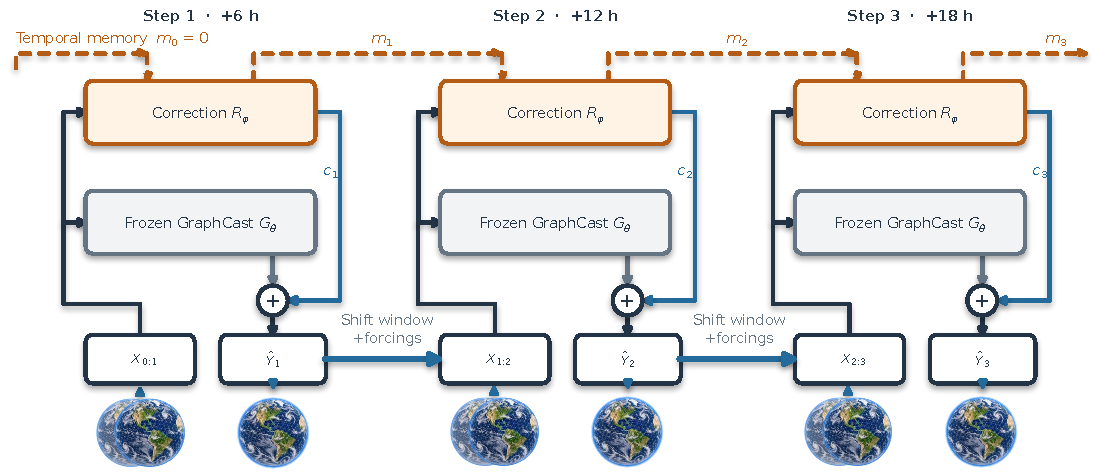
\includegraphics[width=\linewidth]{Pics/gc_mamba_architecture/presentation/03_temporal_rollout.pdf}
        \caption{Autoregressive rollout over three six-hour steps. {Each GraphCast--Mamba forecast advances the two-frame input window; dashed orange arrows carry the temporal memory state}, initialized here with $m_0=0$.}
        \label{fig:GC_Mamba_rollout}
    \end{subfigure}
    \par\smallskip
    \begin{subfigure}{\linewidth}
        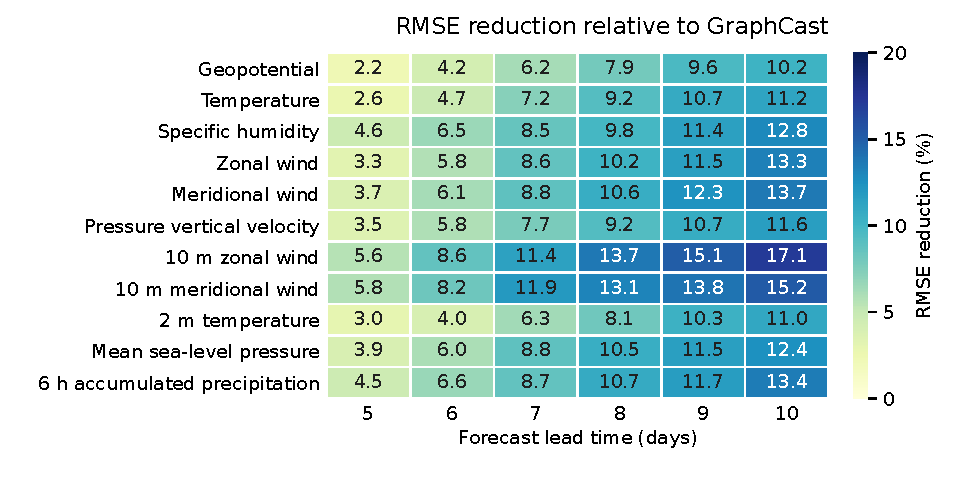
\includegraphics[width=\linewidth]{Graphs/main_v3/overview_7yr_heatmap.pdf}
        \caption{{Variable-group RMSE reductions at days 5 through 10.}}
        \label{fig:breadth_7yr}
    \end{subfigure}
    \par\smallskip
    \begin{subfigure}{\linewidth}
        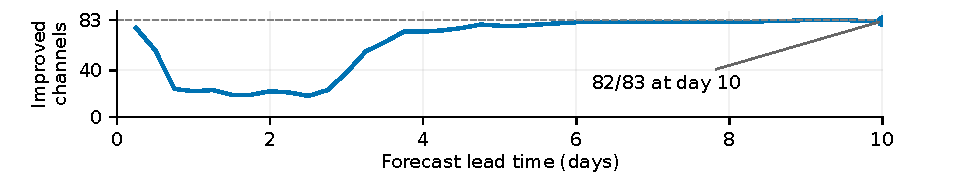
\includegraphics[width=\linewidth]{Graphs/main_v3/overview_7yr_coverage.pdf}
        \caption{{Channel scores: channels with lower RMSE than GraphCast at each six-hour lead.}}
        \label{fig:coverage_7yr}
    \end{subfigure}
    \caption{{GraphCast--Mamba: temporal-memory correction and forecast-skill overview. Panel (a) shows forecast feedback and memory carry. In (b), positive percentages indicate lower variable-group RMSE than the paired GraphCast baseline; (c) counts channels with lower RMSE, out of 83. Counts describe aggregate differences without channel-wise significance tests. Section~\ref{sec:eval_protocol} defines the evaluation protocol and RMSE aggregation.}}
    \label{fig:GC_Mamba}
\end{figure}

\begin{figure}[!htbp]
    \centering
    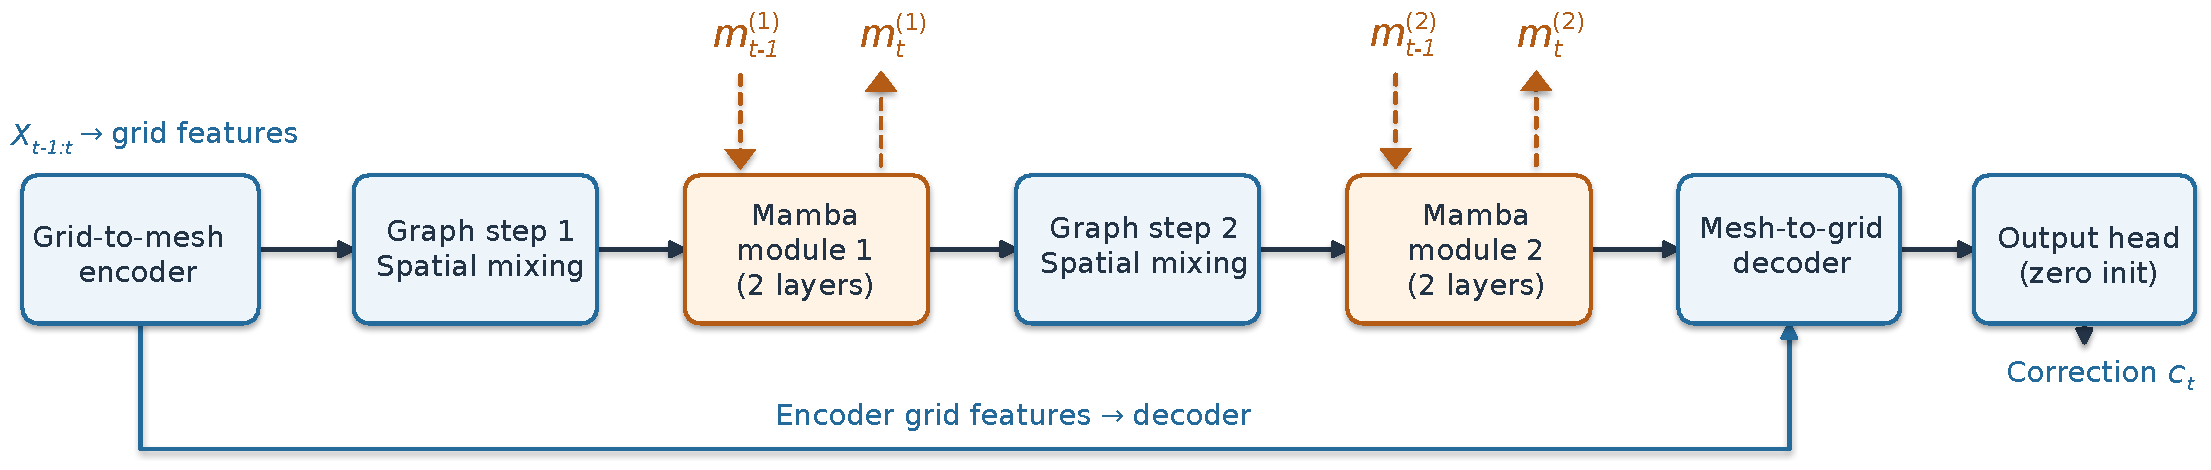
\includegraphics[width=\linewidth]{Pics/gc_mamba_architecture/presentation/02_correction_branch.pdf}
    \caption{{Trainable Mamba correction branch.} Two graph message-passing steps each feed a two-layer Mamba module, followed by decoding and an output head initialized to zero. {The frozen GraphCast backbone forecast $G_\theta(X_t)$ is combined with the learned forecast correction $c_t$ to produce $\hat{Y}_t$. The Mamba correction branch has separate parameters and a temporal memory state $m_t$}, comprising the SSM states and causal-convolution caches of its four Mamba layers.}
    \label{fig:GC_Mamba_correction}
    \vspace{-10pt}
\end{figure}

Our work connects three lines of research: memory-based modeling of partially observed dynamics, temporal memory in weather forecasting, and learned corrections to existing predictors.

\paragraph{Memory and learned closures in reduced dynamics.}
When only part of a dynamical system is resolved, the evolution of the retained variables can depend on their history, as described by the Mori--Zwanzig formalism~\citep{YenTingLinMZ2021}. Motivated by this connection, MemNO combines Fourier neural operators with S4 memory for coarse or noisy PDE observations~\citep{buitrago2025memory}; SS-NO combines spatial state-space operators with temporal memory~\citep{koren2025ssno}. Memory also enters learned corrections to imperfect dynamics: \citet{gupta2021neuralclosures} augment reduced models with neural delay differential equations, while \citet{levine2022modelerror} develop a framework for learning both memoryless and memory-dependent model error. These studies motivate using temporal context to represent effects missing from a predictor's resolved state. Our experiments assess the predictive value of retained context without identifying a physical memory kernel.

\paragraph{Temporal memory in weather forecasting.}
Recurrent weather models already retain information across forecast steps. SwinRNN carries hidden features through global forecasts, while SwinVRNN adds learned perturbations for ensemble prediction~\citep{hu2023swinvrnn}; SwinRDM couples recurrent forecasts with diffusion super-resolution~\citep{chen2023swinrdm}. For radar nowcasting, GauMamba combines Mamba processing with gated recurrent unit (GRU) memory to predict evolving Gaussian representations~\citep{wang2025gaumamba}. These models establish temporal memory as a forecasting mechanism. Our architecture places memory in a separate correction branch: Mamba processes time at each mesh node, graph message passing exchanges spatial information, and the pretrained GraphCast backbone remains frozen.

\paragraph{Learned forecast corrections.}
Learning corrections provides a way to improve an existing predictor while retaining its forecast model. $\delta$-Adapter learns input adjustments and output residual corrections around frozen time-series forecasters~\citep{liang2026forecast}. In numerical weather prediction, \citet{chen2022correcting} learn state-dependent corrections from analysis increments and apply them during FV3-GFS integration. Solver-in-the-Loop trains corrections through differentiable solver rollouts, accounting for their effects on subsequent states~\citep{um2020solver}. These approaches establish both frozen-model adaptation and correction during model integration. For our weather predictor, the remaining question is whether a correction benefits from temporal context beyond the backbone's two-frame input.

These precedents motivate our investigation of persistent temporal memory in a correction branch for a frozen pretrained global weather model. Our experiments compare corrections with and without retained state using the same architecture and parameter count.
\par
\endgroup


% suozhi 原话：图一的a可以加上结果和别的就模型对比 得出我们新模型long horizon很好的结果，需要画图展示这个。
% \suozhi{Please add a results plot to Figure 1(a) comparing our new model with existing models across forecast horizons. The plot should highlight the new model's improvements at long forecast horizons.}
% % suozhi 原话：后面就应该是 method 和 results，这些基本上就是第四面到第九面。
% \suozhi{After Related Work, organize the main text into Method and Results, covering approximately pages four through nine.}

% suozhi 原话：vspace 可以减少白色空白区域。
% \suozhi{Consider using \texttt{\textbackslash vspace} to reduce excess vertical whitespace.}

\section{Method: A hybrid GraphCast--Mamba architecture}

% suozhi 采纳的建议：Method 优先解释本文的训练流程，通用 Mamba 推导可缩短或移到附录。
% \suozhi{Please prioritize the training and inference procedure of our model. Explain which parameters are frozen, how predictions are fed back, when memory is initialized and carried, and where gradients propagate or are stopped. Move these essential details from the appendix into Method. Shorten the general Mamba derivation or move it to the appendix.}

We study whether {a temporal memory state improves forecasts beyond the finite input history supplied to the frozen GraphCast backbone}. GraphCast uses two successive atmospheric states as input; its forecast is Markovian with respect to this augmented state. Figure~\ref{fig:GC_Mamba_rollout} shows {how the Mamba correction branch corrects each GraphCast backbone forecast and carries its temporal memory state across successive six-hour steps. The GraphCast--Mamba forecast advances the meteorological input window, while the temporal memory state retains information from the preceding trajectory.} Figure~\ref{fig:GC_Mamba_correction} details how graph message passing mixes information across mesh nodes and Mamba updates memory independently at each node. This introduces history dependence relative to the baseline input representation.

\subsection{{Architecture}}

\paragraph{{GraphCast backbone}}
{The frozen GraphCast backbone uses a pretrained checkpoint and also serves as the standalone forecast baseline.} This graph neural network operates on a latitude--longitude grid and an auxiliary mesh, with graph $\mathcal{G}(\mathcal{V}^{\textrm{G}},\mathcal{V}^{\textrm{M}},\mathcal{E}^{\textrm{G2M}},\mathcal{E}^{\textrm{M}},\mathcal{E}^{\textrm{M2G}})$. The vertices $\mathcal{V}^{\textrm{G}}$ represent the meteorological grid and $\mathcal{V}^{\textrm{M}}$ the mesh. Encoding uses grid-to-mesh edges $\mathcal{E}^{\textrm{G2M}}$, followed by $N=16$ graph message-passing steps over $\mathcal{E}^{\textrm{M}}$ and decoding over mesh-to-grid edges $\mathcal{E}^{\textrm{M2G}}$. Latent node features have width $W_{\textrm{GC}}=512$. The mesh provides a more compact representation for spatial processing than the meteorological grid.

\paragraph{{Mamba correction branch: temporal memory on the mesh.}}
The Mamba correction branch uses Mamba~\citep{gu2023mamba} to process forecast time independently at each mesh node, with spatial exchange handled by graph message passing. Each layer normalizes the width-$512$ mesh features, projects them into a $d_{\mathrm{inner}}$-dimensional temporal representation, and projects its output back to the mesh width through a residual connection. We use $d_{\mathrm{inner}}=16$. Across autoregressive forecast calls, each layer retains both its {state-space model (SSM) state} and its three-token causal-convolution cache separately for each batch element and mesh node.

Our model uses an SSM state dimension of $16$ per inner channel, a causal convolution width of $4$, a rank-$32$ projection for the step-size parameter $\Delta_t$, and one shared group of input-dependent $B_t,C_t$ coefficients. Additional studies examine $d_{\mathrm{inner}}=32$. The memory-reset controls in Section~\ref{sec:memory_ablation} use $d_{\mathrm{inner}}=16$ and one shared $B,C$ group to test the contribution of temporal memory.


\paragraph{An additive correction with temporal memory.}
Let $X_t$ denote the two-frame meteorological input (shown as $X_{t-1:t}$ in the diagrams) and the associated forcings. Forecast calls are indexed from $t=1$; $\hat{Y}_t$ denotes the next-state forecast produced by call $t$. The temporal memory state $m_t$ collects the SSM states and causal-convolution caches of all Mamba layers. As shown in Figure~\ref{fig:GC_Mamba_rollout}, {GraphCast--Mamba combines the frozen GraphCast backbone $G_\theta$ with the trainable Mamba correction branch $R_\phi$, whose output $c_t$ is the forecast correction}:
\vspace{-4pt}
\begin{equation}
    (c_t,m_t)=R_\phi(X_t,m_{t-1}),
    \qquad
    \hat{Y}_t=G_\theta(X_t)+c_t,
    \qquad \theta\ \text{fixed}.
    \label{eq:additive_correction}
\end{equation}
{The Mamba correction branch in Figure~\ref{fig:GC_Mamba_correction}} has its own grid-to-mesh encoder, mesh processor, and mesh-to-grid decoder. It receives {the same meteorological inputs as the GraphCast backbone} and uses separate parameters throughout. Its mesh processor uses two graph message-passing steps, each followed by a two-layer Mamba module, giving four recurrent layers in total. Encoder grid features are also passed directly to the decoder. Suppressing this grid-feature connection in the notation, the mesh-processing path is
\begin{align}
    L_t^{(0)} &= \operatorname{Encode}_\phi(X_t),\\
    \widetilde{L}_t^{(k)} &= \operatorname{GNN}^{(k)}_\phi(L_t^{(k-1)}),\\
    (L_t^{(k)},m_t^{(k)})
    &=\operatorname{MambaModule}^{(k)}_\phi
       (\widetilde{L}_t^{(k)},m_{t-1}^{(k)}),\qquad k=1,2,\\
    c_t &= \operatorname{Decode}_\phi(L_t^{(2)}).
\end{align}
{Each Mamba module contains two residual Mamba layers; $m_t^{(k)}$ comprises their SSM states and causal-convolution caches.} The output head is initialized to zero, so {the initial GraphCast--Mamba forecast equals the GraphCast backbone forecast}. During autoregressive forecasting, the oldest input frame is dropped, {the GraphCast--Mamba forecast $\hat{Y}_t$ is appended}, and the known forcings are updated to form $X_{t+1}$. {The temporal memory state is passed separately to the next correction-branch call.} The cold-start rollout illustrated in Figure~\ref{fig:GC_Mamba_rollout} begins with $m_0=0$ and {retains the updated temporal memory state thereafter}.


\subsection{Training}
\label{sec:training}
\paragraph{Initialization and trainable parameters.}
The Mamba correction branch inherits pretrained spatial weights and uses a zero-initialized output head, so the initial GraphCast--Mamba forecast matches the GraphCast backbone forecast. We train all correction-branch parameters $\phi$ on ERA5 2015--2021 while keeping the separate GraphCast backbone parameters $\theta$ frozen.

\paragraph{Training segments and memory carry.}
We divide the training sequence into contiguous segments of 96 six-hour steps (24 days), each processed as four consecutive 24-step windows (Figure~\ref{fig:training_segments}). The temporal memory state, comprising both the SSM states and causal-convolution caches, starts at zero for each segment and is carried through all 96 steps. Each window begins with a four-step teacher-forced prefix (ERA5 inputs), followed by 20 feedback-conditioned forecast steps that use the GraphCast--Mamba forecast as feedback. Meteorological inputs therefore return to ERA5 at the start of each window, while the correction branch retains the preceding window's temporal memory state. Gradients propagate through the temporal memory state within a window; at its end, the state is carried forward with its gradient detached. Gradients are also stopped through the meteorological feedback.

\begin{figure}[!htbp]
    \centering
    \normalsize
    \[
    m_{\mathrm{init}}=0\;\longrightarrow\;
    \underbrace{
      \boxed{1{:}24}
      \xrightarrow{\mathrm{sg}}\boxed{25{:}48}
      \xrightarrow{\mathrm{sg}}\boxed{49{:}72}
      \xrightarrow{\mathrm{sg}}\boxed{73{:}96}
    }_{\text{one segment: memory carried through 96 steps}}
    \xrightarrow{\mathrm{reset}}\;m_{\mathrm{init}}'=0
    \]
    \caption{Memory carry during training. Boxes show the four 24-step windows of one segment. The arrows marked $\mathrm{sg}$ carry the SSM states and causal-convolution caches unchanged across window boundaries while stopping their gradients. Both are reset for the next segment.}
    \label{fig:training_segments}
\end{figure}

\paragraph{Training loss.}
At each step, the forecast correction is supervised against the residual target $r_t=Y_t-G_\theta(X_t)$, where $Y_t$ is ERA5 truth and $X_t$ is the current input. Since $c_t-r_t=\hat{Y}_t-Y_t$, this minimizes the {GraphCast loss} $\ell_{\mathrm{GC}}$ of the GraphCast--Mamba forecast. We average the loss over all $H=24$ steps, including the teacher-forced prefix, and the $B$ batch elements:
\begin{equation}
    \mathcal{J}(\phi)
    =\frac{1}{BH}\sum_{b=1}^{B}\sum_{k=1}^{H}
      \ell_{\mathrm{GC}}(\hat{Y}_{b,k},Y_{b,k}).
    \label{eq:training_objective}
\end{equation}
Appendix~\ref{app:training_loss} gives the full loss definition and weights.

\paragraph{Training schedule.}
We train with AdamW for 2,000 post-warm-up updates after a 500-update warm-up, or 2,500 optimizer updates in total. The evaluated model uses stochastic weight averaging (SWA); Appendix~\ref{app:training} gives the detailed configuration, {learning-rate and optimizer comparisons}, and checkpoint-selection procedure.


\section{Results}
\label{sec:numerical}

We evaluate whether GraphCast--Mamba, with its correction branch trained on seven years of ERA5 data (2015--2021), improves on the frozen GraphCast backbone forecasts, how broadly the gains extend across the atmospheric state, and whether temporal memory contributes beyond the correction branch's additional capacity. Separate seven-year memory-reset controls test the contribution of temporal memory.

\subsection{Evaluation protocol and metrics}
\label{sec:eval_protocol}
% suozhi 采纳的建议：用实验概览表统一说明模型、起点、验证网格和指标，区分 loss 与 RMSE 降幅。
% \suozhi{Please add a compact experiment overview table listing the model, forecast starts, verification grid, and metric for each study. Clearly separate the exact GraphCast loss evaluations, the approximate reconstructed loss, and the historical comparison across resolutions. Readers should not assume that every figure uses the same model and evaluation protocol. Consistently distinguish loss reduction from RMSE reduction.}

\begin{figure}[!t]
    \centering
    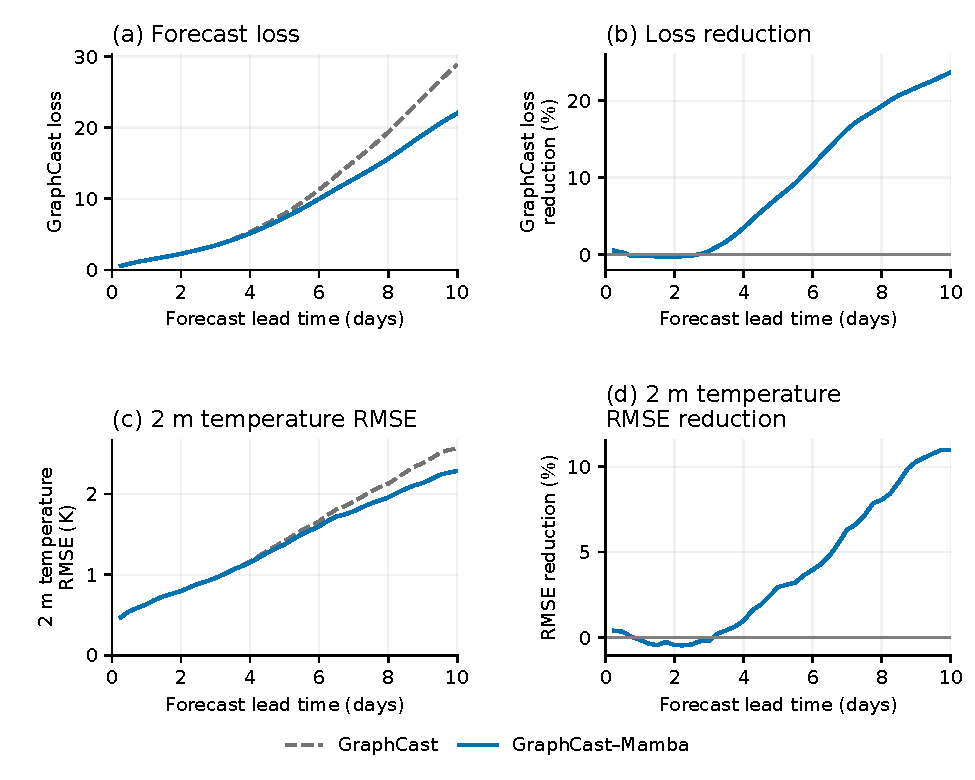
\includegraphics[width=\linewidth]{Graphs/main_v2/exact_gc_loss.pdf}
    \caption{GraphCast--Mamba forecast skill on the evaluation initializations (Section~\ref{sec:eval_protocol}). Top: {GraphCast loss} and its per-lead reduction. Bottom: $2$\,m temperature RMSE and RMSE reduction on the same forecast initializations. The Mamba correction branch uses $d_{\mathrm{inner}}=16$, a threefold Mamba learning rate (LR), and SWA over post-warm-up updates 500--2,000. Every reduction uses the paired GraphCast baseline shown in the absolute-error panels.}
    \label{fig:res1_forecast}
\end{figure}

The principal experiments use GraphCast--Mamba with the original pretrained $1^\circ$ GraphCast backbone and the Mamba correction branch trained in Section~\ref{sec:training}. The same checkpoint supplies the lead-time, variable-group, and channel-coverage results. The principal results use the same 32 forecast initializations drawn at random from the 2022 development set, hereafter the evaluation initializations, on the native $1^\circ$ grid at 40 six-hour forecast steps from 6 to 240\,h. The training schedule and SWA window were fixed before evaluation. The only choice made on these forecast initializations is among the six learning-rate arms in Appendix~\ref{sec:training_sensitivity}. All six reduce the ten-day loss by 14.70--16.34\% and the day-10 loss by 21.98--23.68\%, so the reported gains do not depend on this choice.

Each forecast takes two ERA5 states as input. GraphCast--Mamba initializes the temporal memory state to zero, and advances for ten days using its own predictions as feedback. GraphCast--Mamba feeds back its full prediction, while GraphCast follows an independent uncorrected trajectory. Stateful models retain their updated temporal memory state between steps; the controls without persistent temporal memory reset it at every step.

We first examine aggregate forecast performance using the {GraphCast loss}, with difference-standard-deviation normalization, latitude weights, pressure-level weights, and variable weights. For forecast initializations indexed by $s$, let $\mathcal{L}_{s,k}$ denote this loss at six-hour lead step $k$. The ten-day rollout loss reduction is
\begin{equation}
    \mathcal{I}_{1:40}=100\left(1-
    \frac{\sum_s\sum_{k=1}^{40}\mathcal{L}^{\mathrm{model}}_{s,k}}
         {\sum_s\sum_{k=1}^{40}\mathcal{L}^{\mathrm{GC}}_{s,k}}\right).
    \label{eq:v3_loss_reduction}
\end{equation}
Day-10 loss corresponds to $k=40$ only. Losses are aggregated before taking the ratio; the rollout score is not an average of per-lead percentages.

For each variable and lead, RMSE pools squared physical-unit errors across forecast initializations using normalized cosine-latitude weights before taking the square root. Upper-air variable-group RMSE additionally pools squared errors equally over 13 pressure levels; channel RMSE scores each surface variable and each upper-air pressure level separately. We report $(1-\mathrm{RMSE}_{\mathrm{model}}/\mathrm{RMSE}_{\mathrm{GC}})\times 100\%$, with positive values denoting lower error.

\subsection{Forecast skill improves at longer forecast lead times}

Figure~\ref{fig:res1_forecast} shows that the benefit of the correction is concentrated at longer forecast lead times. Relative to the GraphCast baseline, the {GraphCast loss} decreases by $16.3\%$ over the full ten-day rollout and by $23.68\%$ at the final 240-hour lead.

Physical-unit errors show a similar pattern. For $2$\,m temperature, RMSE remains within $0.5\%$ of the baseline through day 3, before the reduction grows at longer forecast lead times. At day 10, RMSE falls from $2.57$\,K to $2.29$\,K, an $11.0\%$ reduction.


\subsection{Gains extend across the predicted atmospheric state}
{The gains at longer forecast lead times extend across the predicted atmospheric state. All 11 variable groups have lower RMSE at every evaluated six-hour lead from day 5 through day 10, with day-10 reductions of $10.2$--$17.1\%$ (Figure~\ref{fig:breadth_7yr}). These improvements span circulation, thermodynamic, moisture, and surface quantities. Table~\ref{tab:variable_group_rmse} in Appendix~\ref{app:variable_group_rmse} reports the reductions by variable at selected leads, together with absolute day-10 RMSEs.}

% \codexedit{Group-level improvements can conceal deterioration at individual pressure levels. At day 10, 82 of the 83 channels have lower RMSE; the exception is geopotential at 50\,hPa, whose RMSE increases by $1.6\%$ (Figure~\ref{fig:coverage_7yr}). Thus, the gains are broad but do not extend to every channel at the final lead.}

{Appendix~\ref{app:city_traces} complements these aggregate results with individual forecast trajectories at Paris and New York City, including both improvements and larger local errors.}

\subsection{\texorpdfstring{{Comparison with higher-resolution GraphCast}}{Comparison with higher-resolution GraphCast}}
\label{sec:common_grid}
{Figure~\ref{fig:common_grid_selected} compares the GraphCast--Mamba model with its GraphCast backbone and the GraphCast ($0.25^\circ$) reference~\citep{lam2023graphcast} for geopotential at 500\,hPa, $2$\,m temperature, and zonal wind at 850\,hPa. All forecasts are verified on a common $1.5^\circ$ grid. The higher-resolution reference has lower errors at short leads, while GraphCast--Mamba shows slower error growth and achieves lower RMSE at longer forecast lead times in all three quantities. This comparison shows that the learned correction can improve skill at longer forecast lead times even relative to a model with finer output resolution. Appendix~\ref{app:common_grid} provides the complete set of variables.}

\begin{figure}[!htbp]
    \centering
    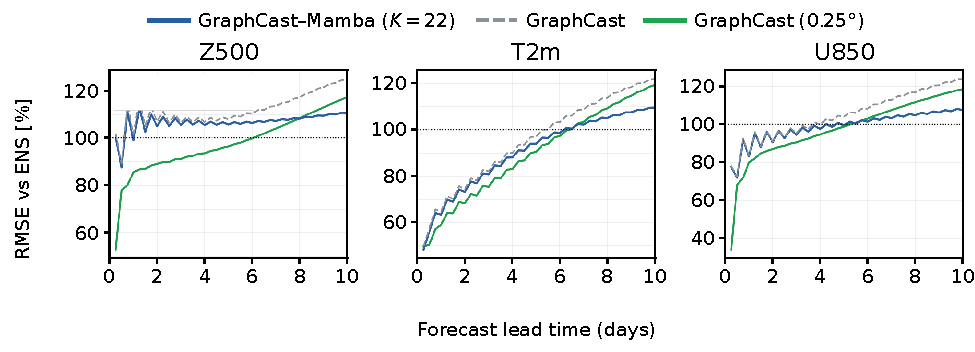
\includegraphics[width=\linewidth]{Graphs/main_v3/common_grid_three_panels.pdf}
    \caption{{Comparison with higher-resolution GraphCast. From left to right: 500\,hPa geopotential (Z500), $2$\,m temperature (T2m), and 850\,hPa zonal wind (U850). Blue shows GraphCast--Mamba model at $1^\circ$, dashed gray its GraphCast baseline, and green the GraphCast ($0.25^\circ$) reference. Forecasts are verified on a common $1.5^\circ$ grid; RMSE is expressed as a percentage of the ECMWF ensemble (ENS) reference, with $100\%$ indicating equal error.}}
    \label{fig:common_grid_selected}
\end{figure}

\subsection{Temporal memory contributes beyond correction capacity}
\label{sec:memory_ablation}
{The preceding results show that GraphCast--Mamba improves forecasts at longer lead times across the predicted atmospheric state. The correction branch introduces both additional trainable capacity and temporal memory. To isolate the contribution of temporal memory in the Mamba correction branch, we test whether retaining this temporal context improves forecasts relative to a correction branch with the same architecture but no persistent temporal memory.}

{Table~\ref{tab:memory_controls} summarizes three policies obtained from two training runs. Policy names specify memory handling during training first and forecasting second. Carry passes the updated SSM state and causal-convolution cache to the next step; reset zeros both before every step. Resetting leaves all learned weights and the two-frame meteorological input in place: the full correction branch still computes a correction, but cannot retain its temporal memory state between calls. Every training segment and independent forecast begins with a zero temporal memory state under all three policies.}

%Note for the future: ideally, we want a unified training framework, not jumping from 2.5k steps to 2-8k.

\begin{table}[!htbp]
    \centering
    \small
    \begin{tabular}{lcc}
        \toprule
        Policy & \multicolumn{2}{c}{Temporal memory retained} \\
        \cmidrule(lr){2-3}
        Training/forecasting & Training & Forecasting \\
        \midrule
        Carry/carry & $\checkmark$ & $\checkmark$ \\
        Carry/reset & $\checkmark$ & $\times$ \\
        Reset/reset & $\times$ & $\times$ \\
        \bottomrule
    \end{tabular}
    \caption{{Memory retained between successive steps: $\checkmark$ denotes retention; $\times$ denotes resetting both the SSM state and causal-convolution cache before every step. Carry/carry and carry/reset share the same trained weights. Reset/reset is trained separately with the same architecture and parameter count.}}
    \label{tab:memory_controls}
\end{table}

{The two training runs use the same seven-year dataset, architecture, optimizer, and training seed, differing in their training/forecasting memory policy. Both use a training tail of $K=20$ feedback-conditioned steps, inner dimension $d_{\mathrm{inner}}=16$. These are separate runs from the principal forecast-skill experiment. We evaluate all three policies on the forecast initializations and lead times of Section~\ref{sec:eval_protocol}. {Appendix~\ref{app:training_loss} describes the loss calculation for these controls.}}

\begin{figure}[!htbp]
    \centering
    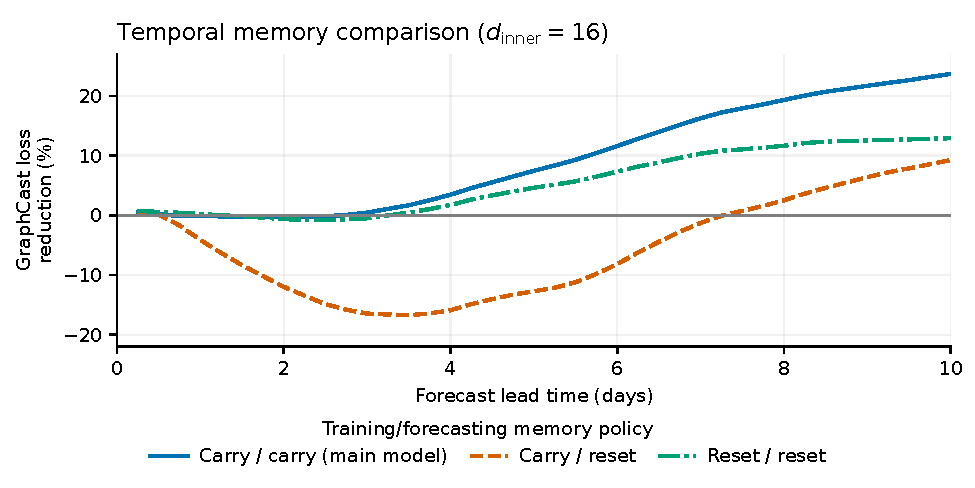
\includegraphics[width=0.8\linewidth]{Graphs/main_v3/memory_reset_main_model.pdf}
    \caption{{\textbf{Comparison of carry/carry, carry/reset, and reset/reset memory policies defined in Table~\ref{tab:memory_controls}.} Curves show GraphCast loss reduction relative to each model's paired GraphCast baseline over ten forecast days.}}
    \label{fig:memory_reset}
\end{figure}


% suozhi 采纳的建议：突出记忆对照，用表格区分训练与预测时的状态策略，并明确 SSM 与卷积缓存的归因边界。
% \suozhi{Please give the memory controls a more prominent role in the argument. A small table should show whether carry/carry, carry/reset, and reset/reset retain memory during training and forecasting, and which control is trained separately. Explain how the controls distinguish additional model capacity from persistent memory. Since resetting clears both the SSM state and convolution cache, the current study does not isolate the contribution of long-term SSM memory.}

The memory controls distinguish reliance on the temporal memory state from the benefit of training with persistent temporal memory (Table~\ref{tab:memory_controls}). In the separate control runs, resetting the memory-trained model during forecasting (carry/reset) reduces the day-10 {GraphCast loss} reduction from {$23.68\%$} to $9.24\%$. This shows that the model uses its temporal memory state, although the drop may partly reflect the mismatch between training and forecasting. Training the correction with its temporal memory state reset at every step (reset/reset) removes this mismatch and yields a $12.91\%$ reduction with the same architecture and parameter count. The control run's carry/carry policy therefore improves on a correction trained without persistent temporal memory by {$10.77$} percentage points, supporting a benefit from temporal context beyond additional trainable capacity. Figure~\ref{fig:memory_reset} shows the principal model's {carry/carry curve in place of the control run's carry/carry curve}; its comparison with the reset controls also includes differences in training configuration and loss measurement.

Together, the two comparisons show that the memory-trained model uses its temporal memory state and outperforms the separately trained control without persistent temporal memory in this setting. This supports useful history dependence beyond the baseline's two-frame input.

\section{Conclusion}

Our results show that a small correction branch with persistent temporal memory can improve forecasts from a frozen pretrained weather model at longer forecast lead times. Memory controls support a benefit from retained history beyond the branch’s additional trainable capacity. This suggests that compact temporal extensions offer a promising way to improve existing forecasters with limited additional training. How this benefit depends on spatial resolution and the choice of backbone remains an open question.

{\textbf{Limitations.} Deterministic AI weather models can produce overly smooth fields and struggle to predict extremes despite good average skill. \citet{zhang2025numerical} discuss this smoothing tendency and find that several leading models underestimate the frequency and intensity of record-breaking heat, cold, and wind events. We have not systematically evaluated whether GraphCast--Mamba reduces smoothing or improves extreme-event prediction. The aggregate loss and RMSE reductions reported here therefore do not establish improved skill for rare extremes.}
% Keep all main-text floats ahead of the references and appendices.
\FloatBarrier


% ICLR 2027 requires an AI use statement, excluded from the page limit.
% AUTHOR TODO: Add a statement reflecting the full study-wide history and the
% authors' verification. Template migration and manuscript review used AI.
% V3 AUTHOR TODO: Verify the statement below against the full study-wide history
% and document the authors' checks before submission.
% Keep this as an author action rather than inserting unapproved manuscript prose.
\clearpage
\section*{AI use statement}

We used a large language model for minor editorial assistance, including correcting grammar and
typo and refining formatting. It did not contribute to the development of research ideas, the analysis,
or the claims.

\section*{Ethics Statement}
All datasets, models in this work are publicly available. The usage of these datasets, models, code strictly follows the terms and conditions set by the providers. 

\section*{Reproducibility Statement}
To ensure reproducibility of our results, we provide detailed documentation of our experimental setup and methodology in the main paper and appendix. The code for data, evaluation,
and training will be open-sourced upon publication.


% suozhi 原话：我们最后需要 AI statement。
% \suozhi{We need to include an AI use statement before submitting the paper.}

\bibliographystyle{iclr2027_conference}
\bibliography{bib}

\clearpage
\appendix

\section{\texorpdfstring{{Training details and model selection}}{Training details and model selection}}
\label{app:training}

\subsection{Training configuration}
\label{app:training_configuration}
The configuration below supplies the principal {GraphCast loss} and RMSE results in Section~\ref{sec:numerical}.

\paragraph{Initialization and batching.}
We initialize the Mamba correction branch from the frozen GraphCast backbone checkpoint: its grid-to-mesh encoder (G2M), mesh-to-grid decoder (M2G), and two graph message-passing steps copy the corresponding pretrained weights, using the first two of GraphCast's 16 graph message-passing steps. We insert newly initialized Mamba modules after these graph message-passing steps and append a linear output head with weights and biases initialized to zero. Consequently, the initial forecast correction is zero and the GraphCast--Mamba forecast equals the pretrained GraphCast backbone forecast. The copied spatial parameters, Mamba modules, and output head form the trainable parameters $\phi$; the separate GraphCast backbone parameters $\theta$ remain frozen throughout training on ERA5 2015--2021. Each optimizer update processes one window from each of four independent segments, giving batch size $B=4$ under the memory-carry procedure in Section~\ref{sec:training}.

\paragraph{Optimizer and checkpoint settings.}
The reported model uses a 500-update warm-up followed by 2,000 post-warm-up updates. We use AdamW with moments $(0.9,0.98)$ and a base peak learning rate of $10^{-4}$; the Mamba parameters receive three times the spatial learning rate. The evaluated model averages the parameters saved at post-warm-up updates 500, 1,000, 1,500, and 2,000 using SWA. These checkpoint indices count updates after warm-up. The configuration uses spatial width 512, inner dimension 16, and one $B,C$ group.

\subsection{Complete loss definition}
\label{app:training_loss}
The per-step loss in Equation~\ref{eq:training_objective} is the {GraphCast loss}:
\begin{equation}
    \ell_{\mathrm{GC}}(\hat{Y},Y)
    =\sum_v\frac{\lambda_v}{N_{\mathrm{g}}L_v}
      \sum_{i=1}^{N_{\mathrm{g}}}\sum_{\ell=1}^{L_v}
      a_i q_{v,\ell}
      \left(\frac{\hat{Y}_{v,\ell,i}-Y_{v,\ell,i}}
      {\sigma_{v,\ell}}\right)^2.
    \label{eq:training_gc_loss}
\end{equation}
Here $N_{\mathrm{g}}$ is the number of grid points and $L_v$ is the number of levels for variable $v$. The scales $\sigma_{v,\ell}$ are GraphCast's standard deviations of six-hour differences. The latitude weights $a_i$ have unit mean and include the pole-cell correction. For upper-air variables, $q_{v,\ell}=p_\ell/\overline{p}$ weights levels in proportion to pressure; surface variables have $L_v=1$ and $q_{v,1}=1$. The variable weights $\lambda_v$ are 1 for upper-air variables and $2$\,m temperature, and 0.1 for the two $10$\,m wind components, mean sea-level pressure, and six-hour accumulated precipitation.

\paragraph{{Evaluation variants.}}
{We use GraphCast loss as the common label for the weighted MSE diagnostics. The principal results evaluate Equation~\ref{eq:training_gc_loss} directly. The memory controls and closed-loop training-tail sweep reconstruct it from channel RMSEs using per-level normalization and pressure weights, without the pole-cell correction. The archived open-loop sweep instead uses variable-group RMSEs and level-averaged normalization scales. These reconstructions therefore approximate the loss above.}



\subsection{\texorpdfstring{{Mamba capacity and learning-rate selection}}{Mamba capacity and learning-rate selection}}
\label{sec:training_sensitivity}
% Parameter counts: artifacts/checkpoints/v24_Ilya/res1_batch4_temporal_lr_20260908/
% runs/{di16_fast_mamba,di32_joint}/run_config.json, derived:
% mamba_parameters = 110016 / 215936; spatial_parameters = 10238863.
{Learning-rate choice depends on network width and parameterization. \citet{yang2022tensorprogramsv} derive width-dependent scaling rules under maximal update parameterization ($\mu$P), including an inverse-width scaling for Adam learning rates on hidden weight matrices. In our correction branch, the newly initialized Mamba modules contain approximately 0.11M and 0.22M parameters at inner dimensions 16 and 32, respectively, compared with 10.24M parameters in the spatial components. Motivated by these scaling results and the difference in module size, we test whether the compact Mamba modules benefit from a larger learning rate than the spatial components initialized from pretrained GraphCast weights. We treat this as an empirical hypothesis; the $\mu$P scaling rule does not directly prescribe a learning-rate multiplier for our architecture.}

{We compare Mamba learning-rate multipliers of $0.3\times$, $1\times$, and $3\times$ at each inner dimension, holding the spatial peak learning rate fixed at $10^{-4}$. A multiplier of $1\times$ gives equal learning rates to both parameter groups. All six configurations use spatial width 512, one $B,C$ group, batch size four, and AdamW moments $(0.9,0.98)$. Each run has its own 500-update warm-up followed by 2,000 post-warm-up updates, with SWA over post-warm-up updates 500, 1,000, 1,500, and 2,000. The GraphCast backbone remains frozen throughout. Warm-up parameter values differ across runs despite the common training seed, so the comparisons assess complete training runs.}

\begin{table}[!htbp]
    \centering
    \caption{Mamba capacity and learning-rate comparison at $1^\circ$. Entries are {GraphCast loss} reductions (\%) on the evaluation initializations (Section~\ref{sec:eval_protocol}); bold marks the largest value in each metric column. The multiplier applies only to Mamba parameters, with the spatial learning rate fixed. All six configurations use the same training schedule and SWA window.}
    \label{tab:lr_sensitivity}
    \small
    \begin{tabular}{rrrr}
        \toprule
        $d_{\mathrm{inner}}$ & Mamba LR multiplier & Ten-day aggregate & Day 10 \\
        \midrule
        16 & $0.3\times$ & 14.70 & 21.98 \\
        16 & $1\times$   & 15.67 & 22.44 \\
        16 & $3\times$   & \textbf{16.34} & \textbf{23.68} \\
        32 & $0.3\times$ & 15.82 & 22.96 \\
        32 & $1\times$   & 16.29 & 23.32 \\
        32 & $3\times$   & 15.73 & 22.75 \\
        \bottomrule
    \end{tabular}
\end{table}

\begin{samepage}
Table~\ref{tab:lr_sensitivity} shows that, for inner dimension 16, increasing the Mamba learning-rate multiplier from $1\times$ to $3\times$ raises the ten-day aggregate loss reduction from $15.67\%$ to $16.34\%$ and the day-10 reduction from $22.44\%$ to $23.68\%$. For inner dimension 32, the best tested multiplier is $1\times$; increasing it to $3\times$ lowers the aggregate reduction from $16.29\%$ to $15.73\%$. Dimension 32 performs better at $0.3\times$ and $1\times$, whereas dimension 16 performs better at $3\times$. Thus, the smaller GraphCast-Mamba head benefits from a larger learning rate in these runs, supporting joint selection of Mamba capacity and learning rate. The results do not establish a monotonic benefit from increasing either quantity.\par
\end{samepage}

\subsection{\texorpdfstring{{Optimizer configuration study}}{Optimizer configuration study}}
\label{app:optimizer_study}
The optimizer study varies peak learning rate ($10^{-4}$ or $5\times10^{-5}$), Adam moments, Mamba initialization scheme (legacy or Mamba1), and the paired inner-dimension/group settings (16/1 or 64/4). The latter changes two factors simultaneously and does not isolate inner dimension. Runs use 10,000 updates, seed 22, a 200-update warm-up, cosine decay to one tenth of the peak learning rate, and weight decay $10^{-4}$. {The correction branch is trained} with closed-loop feedback, 24-step backpropagation windows, a training tail of 20 feedback-conditioned steps, and loss across all 24 steps. {The forecast correction contribution to the feedback} is stop-gradient, while temporal memory state gradients propagate within the backpropagation window.

Day-10 reductions for the 22 completed selected SWA configurations range from $13.47\%$ to $23.21\%$. The configuration at the upper end uses Mamba1 initialization, inner dimension 16, one $B,C$ group, learning rate $10^{-4}$, and AdamW moments $(0.9,0.98)$; its aggregate loss reduction is $16.28\%$.

\subsection{\texorpdfstring{{Checkpoint averaging and model selection}}{Checkpoint averaging and model selection}}
\label{app:checkpoint_selection}
\begin{samepage}
\paragraph{Stochastic weight averaging.}
{SWA averages correction-branch parameter values} from saved checkpoints to reduce dependence on a single training iterate \citep{izmailov2019averagingweightsleadswider}. Every configuration in {Table~\ref{tab:lr_sensitivity}} averages four checkpoints at {post-warm-up updates} 500, 1,000, 1,500, and 2,000. The dimension-16 Mamba1-initialized optimizer-study configuration described above averages seven checkpoints, saved every 1k updates from 2k through 8k. These are parameter averages, not ensembles of independent forecast predictions. {Evaluation initializes the temporal memory state to zero}, including for SWA models.
\end{samepage}

\paragraph{Training methods and model selection.}
{Table~\ref{tab:lr_sensitivity} reports all six SWA configurations from the Mamba capacity and learning-rate comparison.} Figure~\ref{fig:res1_forecast} uses the dimension-16, $3\times$ Mamba learning-rate SWA configuration, which has the largest aggregate and day-10 {GraphCast loss} reductions among the completed SWA configurations in the reported optimizer and learning-rate studies.

{In the optimizer study, each run screens periodic checkpoints and three SWA windows on eight forecast initializations.} The selected checkpoint and SWA are then evaluated on the evaluation initializations.

\subsection{Variable-group RMSE}
\label{app:variable_group_rmse}

Table~\ref{tab:variable_group_rmse} provides the numerical results underlying Figure~\ref{fig:breadth_7yr} at selected forecast leads. It uses the principal seven-year correction and its paired GraphCast baseline on the 32 development-set forecast initializations in 2022, evaluated on the native $1^\circ$ grid as described in Section~\ref{sec:eval_protocol}.

\begin{table}[!htbp]
    \centering
    \small
    \setlength{\tabcolsep}{4pt}
    % Source: Graphs/main_v3/breadth_7yr_all_leads.csv, leads 120/168/240 h.
    % Absolute RMSE conversions: humidity kg/kg -> g/kg (x1000),
    % sea-level pressure Pa -> hPa (/100), precipitation m -> mm (x1000).
    % Reductions use unrounded RMSEs; pressure velocity retains three decimals.
    \begin{tabular}{@{}lrrrrr@{}}
        \toprule
        & \multicolumn{2}{c}{Day-10 RMSE} & \multicolumn{3}{c}{RMSE reduction (\%)} \\
        \cmidrule(lr){2-3}\cmidrule(l){4-6}
        Variable [unit] & GraphCast & \shortstack{GraphCast--\\Mamba} & Day 5 & Day 7 & Day 10 \\
        \midrule
        \multicolumn{6}{@{}l}{\textit{Upper-air variables (13 pressure levels)}} \\
        Geopotential [m$^2$\,s$^{-2}$] & 774.74 & 695.67 & 2.23 & 6.16 & 10.21 \\
        Temperature [K] & 3.10 & 2.76 & 2.59 & 7.24 & 11.22 \\
        Specific humidity [g\,kg$^{-1}$] & 1.08 & 0.94 & 4.64 & 8.48 & 12.83 \\
        Zonal wind [m\,s$^{-1}$] & 8.69 & 7.53 & 3.28 & 8.60 & 13.35 \\
        Meridional wind [m\,s$^{-1}$] & 9.06 & 7.82 & 3.69 & 8.75 & 13.66 \\
        \shortstack[l]{Pressure vertical velocity\\{}[Pa\,s$^{-1}$]} & 0.154 & 0.136 & 3.46 & 7.67 & 11.60 \\
        \addlinespace
        \multicolumn{6}{@{}l}{\textit{Surface variables}} \\
        $10$\,m zonal wind [m\,s$^{-1}$] & 4.31 & 3.57 & 5.56 & 11.37 & 17.06 \\
        $10$\,m meridional wind [m\,s$^{-1}$] & 4.48 & 3.80 & 5.78 & 11.90 & 15.18 \\
        $2$\,m temperature [K] & 2.57 & 2.29 & 2.96 & 6.32 & 10.98 \\
        Mean sea-level pressure [hPa] & 7.16 & 6.27 & 3.87 & 8.80 & 12.42 \\
        \shortstack[l]{$6$\,h accumulated\\precipitation [mm]} & 2.35 & 2.04 & 4.54 & 8.66 & 13.44 \\
        \bottomrule
    \end{tabular}
    \caption{Physical-unit RMSE and relative RMSE reduction for the principal GraphCast--Mamba model. Days 5, 7, and 10 denote leads of 120, 168, and 240\,h. RMSE pools cosine-latitude-weighted squared errors across forecast initializations and, for upper-air groups, equally across 13 pressure levels before taking the square root. Each reduction is $100(1-\mathrm{RMSE}_{\mathrm{model}}/\mathrm{RMSE}_{\mathrm{GC}})$, computed before rounding. Positive values indicate lower RMSE; these percentages are distinct from GraphCast loss reductions.}
    \label{tab:variable_group_rmse}
\end{table}

\clearpage
\section{Training tail length}
\label{app:training_horizon}

We examine how forecast skill depends on the training tail length $K$ under two input-feedback policies. Each 24-step training window begins with a \emph{teacher-forced prefix}: the model receives ERA5 states as meteorological inputs while updating and retaining its temporal memory. For $K>1$, the final $K$ steps instead use forecast feedback, leaving $24-K$ teacher-forced steps. The label $K=1$ denotes fully teacher-forced training, with ERA5 inputs at every step. We evaluate the resulting models over 40 six-hour forecast steps (ten days) and report {GraphCast loss} reduction relative to GraphCast; positive values indicate improved forecast skill.

\subsection{Closed-loop training(our main model)}
In \emph{closed-loop training}, the corrected GraphCast--Mamba forecast supplies the next meteorological input during the training tail. The learned correction therefore affects both the current prediction and the inputs encountered at subsequent steps. Figure~\ref{fig:training_horizon_closed_loop} compares models trained with different $K$, showing how the duration of this feedback changes forecast skill.

\begin{figure}[!htbp]
    \centering
    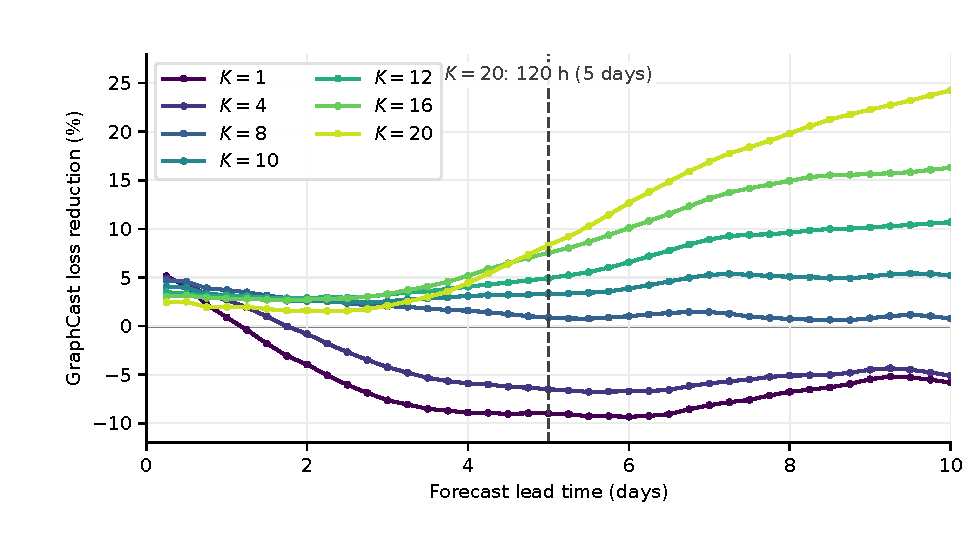
\includegraphics[width=\linewidth]{Graphs/main_v3/training_ar_horizon_15yr_closedloop.pdf}
    \caption{Forecast skill after closed-loop training with different training tail lengths $K$. During the tail, corrected GraphCast--Mamba predictions supply subsequent inputs. Each curve shows {GraphCast loss} reduction relative to GraphCast over ten forecast days; positive values indicate improvement. \textcolor{blue}{The vertical dashed line marks $20\times6=120$\,h (5 days), the training tail duration for $K=20$. Gains for this model persist beyond its training tail to day 10, twice that duration.}}
    \label{fig:training_horizon_closed_loop}
\end{figure}

Short training tails primarily improve early forecasts. Models trained with $K=1$ and $K=4$ reduce error during the first one to two days but increase it thereafter, whereas longer training tails yield substantial gains at longer lead times. At day 10, the error reduction relative to GraphCast increases from 5.2\% for $K=10$ to 24.3\% for $K=20$. These curves reveal a crossover: shorter tails favor early forecast skill, while longer tails become more effective as the forecast advances. To examine this crossover in a more controlled setting, we remove correction feedback and train the Mamba correction branch on precomputed forecast trajectories from the frozen GraphCast backbone. In this open-loop setting, corrections do not affect subsequent backbone predictions. As shown in the next section, the crossover becomes more pronounced under this training scheme.

\clearpage
\subsection{Open-loop training and a sharper crossover}
In \emph{open-loop training}, the teacher-forced prefix is followed by a tail driven by the uncorrected GraphCast forecasts. The correction branch learns along this trajectory, but its predictions do not alter subsequent meteorological inputs. Thus, open loop refers to the absence of correction feedback, while teacher forcing refers to the use of ERA5 inputs in the prefix.

In our experiments, training with this teacher-forced prefix and a tail independent of the learned correction was more stable but {yielded smaller improvements at longer lead times}. Figure~\ref{fig:training_horizon_open_loop} shows that short-tail models remain close to GraphCast at long lead times, avoiding the substantial degradation seen in the closed-loop comparison. The crossover is more pronounced here: long-lead gains change markedly between $K=16$ and $K=18$ and increase further for $K=20$ and $K=22$.

\begin{figure}[!htbp]
    \centering
    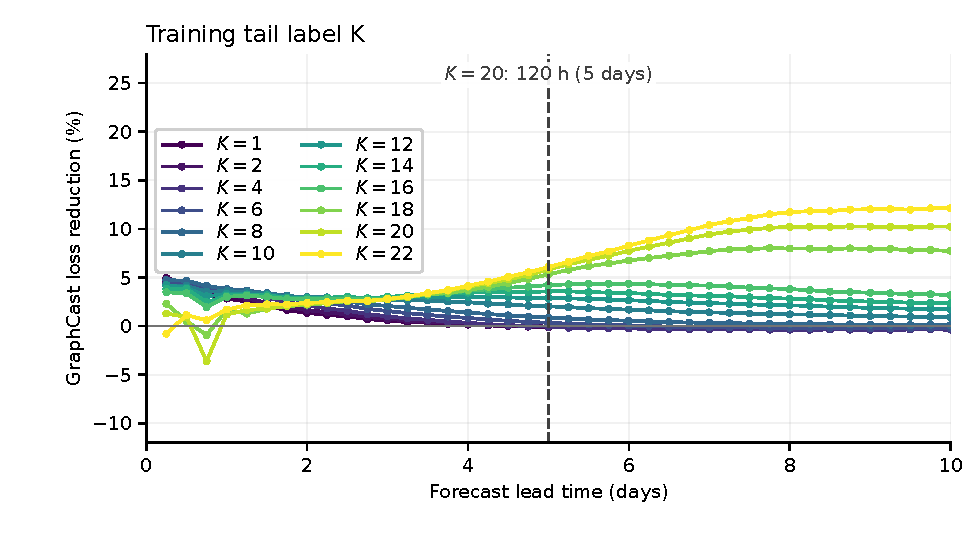
\includegraphics[width=\linewidth]{Graphs/main_v2/training_ar_horizon.pdf}
    \caption{Forecast skill after open-loop training with a teacher-forced prefix and different training tail lengths $K$. During the tail, uncorrected GraphCast forecasts supply subsequent inputs. {GraphCast loss} reduction exhibits a pronounced crossover, with substantially larger long-lead gains for $K\geq18$. {\textcolor{blue}{The vertical dashed line marks $20\times6=120$\,h (5 days), the training tail duration for $K=20$; this model retains positive gains beyond that duration, up to day 10.} This figure and Figure~\ref{fig:training_horizon_closed_loop} use the same vertical scale but compare separate sweeps with different experimental settings and loss reconstructions (Appendix~\ref{app:training_loss}).}}
    \label{fig:training_horizon_open_loop}
\end{figure}

This crossover raises an interesting question about how temporal memory, training tail length, and feedback interact. Its mechanism, including why it is sharper under open-loop training, remains unclear. We regard it as an empirical finding that motivates further investigation, rather than evidence for a universal critical value of $K$.


\clearpage

\section{Comparison on a common verification grid}
\label{app:common_grid}
\begin{figure}[!t]
    \centering
    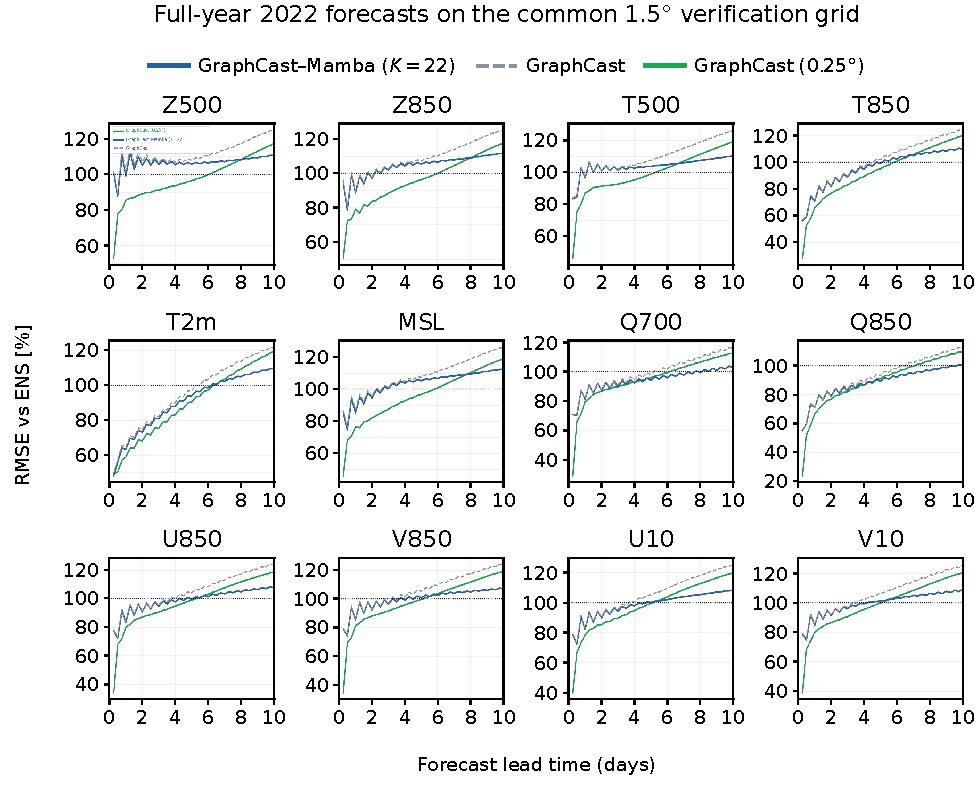
\includegraphics[width=\linewidth]{Graphs/add_mamba.pdf}
    \caption{Complete common-grid comparison. The quantities span geopotential, temperature, mean sea-level pressure, specific humidity, and wind. The panel labels use Z for geopotential, T for temperature, Q for specific humidity, U for zonal wind, and V for meridional wind; a three-digit suffix gives pressure in hPa. T2m denotes $2$\,m temperature, U10 and V10 denote the $10$\,m wind components, and MSL denotes mean sea-level pressure. Blue is our GraphCast--Mamba model at $1^\circ$ and $K=22$, dashed gray its GraphCast baseline, and green GraphCast ($0.25^\circ$). Forecasts are verified on a common $1.5^\circ$ grid, with RMSE normalized to the ECMWF ensemble (ENS) reference ($100\%$ denotes equal RMSE).{Figure~\ref{fig:common_grid_selected} presents three representative quantities in the main text.}}
    \label{fig:res1_all_variables}
\end{figure}


We further assess forecast skill for the meteorological quantities shown in Figure~\ref{fig:res1_all_variables}, following the variables considered in the original GraphCast study~\citep{lam2023graphcast}. Although the models operate at different native spatial resolutions, all forecasts are projected and evaluated on the same $1.5^\circ$ verification grid, so that the comparison reflects forecast accuracy rather than differences in verification resolution. Across these variables, our $1^\circ$ GraphCast--Mamba model exhibits slower error growth with forecast lead time than its uncorrected GraphCast baseline. Remarkably, at longer lead times it also attains lower errors than the GraphCast ($0.25^\circ$) reference, despite operating at a substantially coarser native resolution. The GraphCast ($0.25^\circ$) reference itself was trained with considerable computational resources, approximately four weeks on 32 TPU v4 devices~\citep{lam2023graphcast}.

\clearpage
\section{Forecast examples at city locations}
\label{app:city_traces}
To complement the aggregate seven-year results in Section~\ref{sec:numerical}, Figure~\ref{fig:city_traces_jan} illustrates local forecast behavior for temperature, wind, and precipitation at Paris and New York City. These examples use a separate correction trained on 15 years of ERA5 data (2007--2021), with the configuration specified in the figure caption. Over 120--240\,h, the correction reduces mean absolute error (MAE) in four of the six displayed city--variable pairs. Errors increase for Paris temperature and New York precipitation, illustrating that aggregate skill gains can coexist with deterioration in individual forecasts.

\begin{figure}[!htbp]
    \centering
    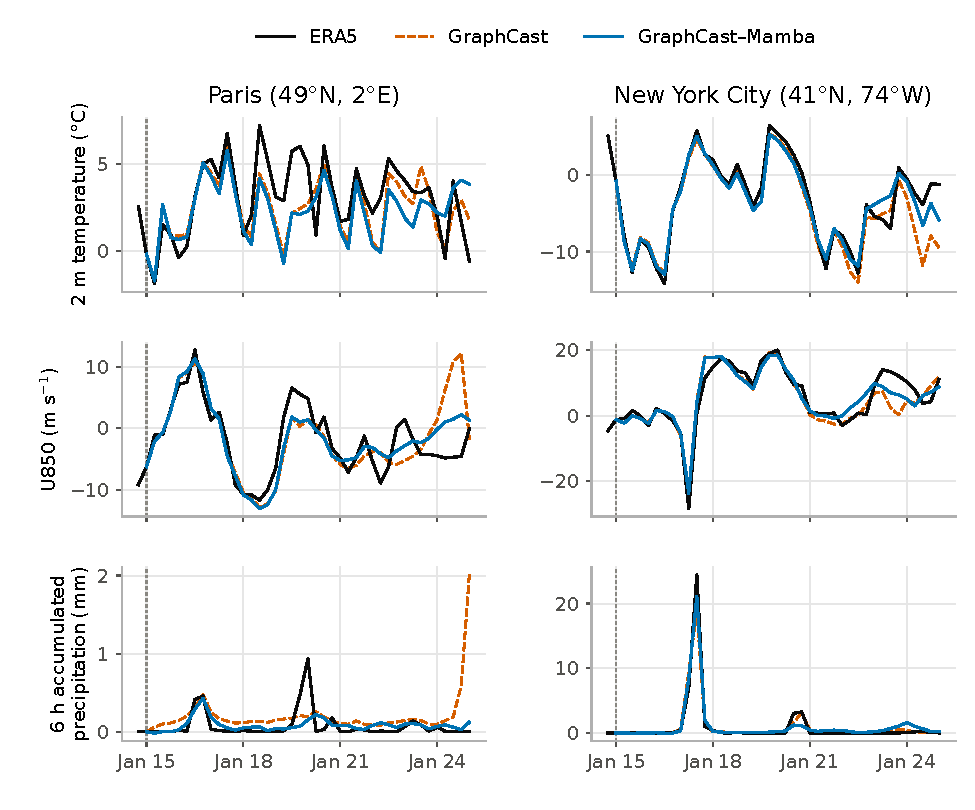
\includegraphics[width=\linewidth]{Graphs/city_traces/cities_Paris_NYC_20220115_compact.pdf}
    \caption{{Ten-day forecasts from 00\,UTC on 15 January 2022 at the $1^\circ$ grid points nearest Paris ($49^\circ$N, $2^\circ$E; left) and New York City ($41^\circ$N, $74^\circ$W; right).
    From top to bottom, rows show $2$\,m temperature (T2m), $850$\,hPa zonal wind (U850), and $6$\,h accumulated precipitation in physical units.
    ERA5 is shown in black, the frozen GraphCast forecast in dashed orange, and the GraphCast--Mamba forecast in blue.
    The correction was trained separately on 15 years of ERA5 data (2007--2021), with a training tail of $K=20$ feedback-conditioned steps, Mamba inner dimension $128$, spatial width $512$, and two graph message-passing steps; SWA averages checkpoints from updates 6k--11k.
    Both forecasts use the ERA5 states at $-6$ and $0$\,h (before and on the dotted line) as inputs, then feed back their own predicted fields at each step; the GraphCast--Mamba model begins with a zero temporal memory state.
    Precipitation is shown as predicted and may take small negative values.}}
    \label{fig:city_traces_jan}
\end{figure}


\end{document}
